\documentclass[10pt,a4paper]{amsart}
\usepackage[margin=19mm]{geometry}
\usepackage{amsmath,amssymb,mathtools}
\usepackage[scr=rsfs,cal=euler]{mathalfa}
\usepackage{xfrac}
\usepackage[unicode,hidelinks,bookmarks=false]{hyperref}
\newcommand{\ie}{i.e.\ }
\newcommand{\cf}{cf.\ }
\newcommand{\resp}{respectively\ }
\newcommand{\Subsection}{\subsection}
\providecommand{\nobreakdash}{\nobreak\hbox{-}}
\setlength{\emergencystretch}{2em}
\multlinegap0pt
\usepackage{tikz}
\usepackage{enumerate}
\usepackage{amssymb}
\newtheorem{lem}{Lemma}
\title{Higher-dimensional symbolic dynamics: A textile framework for $3$-graphs}
\author{Roozbeh Hazrat, Promit Mukherjee, Sujit Kumar Sardar}
\date{Source: arXiv:2607.29233v1 (CC BY 4.0)}
\begin{document}
\maketitle

\noindent\emph{Source and licence.} Higher-dimensional symbolic dynamics: A textile framework for $3$-graphs. Version arXiv:2607.29233v1 (CC BY 4.0), distributed by arXiv under the Creative Commons Attribution 4.0 International licence, http://creativecommons.org/licenses/by/4.0/, as recorded in the arXiv licence metadata for this exact version and shown on the abstract page https://arxiv.org/abs/2607.29233v1. Full licence notice: \texttt{licenses/arxiv-2607.29233-CC-BY-4.0.txt}.\par\smallskip

\noindent\textit{Editorial scope.} Counted unit: the article's lem pullbacks (source0.tex lines 1832--1955). The article's complete original proof of it is delivered with it (source0.tex lines 1956--2144, one \texttt{proof} environment of 189 lines). No mathematics is written, repaired or re-derived: the statement and the proof are the article's own lines, in the article's own notation, and no retained line is substituted or re-flowed.  No further source-local context is needed: every cross-reference of every retained line resolves inside the two delivered spans.  Nothing was omitted from any retained span, so the package carries no omission record.  No retained line contains a citation, so the wrapper carries no bibliography and no bibliography entry.  The retained lines contain the article's own diagram code, which the wrapper typesets with the standard tikz packages; no image file is delivered and the package declares no asset dependency.  Editorial formatting only, in addition: an AMS \texttt{amsart} preamble that restates the article's own declarations and macros used by the retained lines, namely the environments \texttt{lem} on separate counters, together with the standard packages those lines need.  The retained environments print in this document as Lemma 1 in order of appearance, whereas the article prints the same items with the numbering of its own full document.  The complete native source of the article as distributed in the arXiv e-print for this exact version is bundled unchanged as \texttt{sources/206465/source0.tex}.
\begin{lem}\label{lem other pullbacks}
Let $\mathcal{T}$ be a three-dimensional textile presented by the following diagram: 

\[
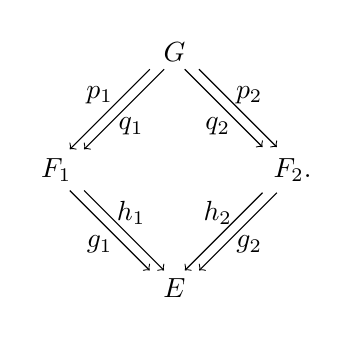
\begin{tikzpicture}[scale=1]
\node[inner sep=2.5pt, circle] (B) at (-1.5,0) {$F_1$};
\node[inner sep=2.5pt, circle] (C) at (1.5,0) {$F_2.$};	
\node[inner sep=2.5pt, circle] (D) at (0,-1.5) {$E$};
\node[inner sep=2.5pt, circle] (A) at (0,1.5) {$G$}; 

\draw[transform canvas={xshift=0.6ex}, ->] (A) -- (B);
\draw[transform canvas={xshift=-0.6ex}, ->] (A) -- (B);

\draw[transform canvas={xshift=0.6ex}, ->] (A) -- (C);
\draw[transform canvas={xshift=-0.6ex}, ->] (A) -- (C);

\draw[transform canvas={xshift=0.6ex}, ->] (C) -- (D);
\draw[transform canvas={xshift=-0.6ex}, ->] (C) -- (D);

\draw[transform canvas={xshift=0.6ex}, ->] (B) -- (D);
\draw[transform canvas={xshift=-0.6ex}, ->] (B) -- (D);

\node at (-0.55,0.55) {$q_1$};
\node at (-0.95,0.95) {$p_1$};

\node at (0.55,0.55) {$q_2$};
\node at (0.95,0.95) {$p_2$};

\node at (-0.55,-0.55) {$h_1$};
\node at (-0.95,-0.95) {$g_1$};

\node at (0.55,-0.55) {$h_2$};
\node at (0.95,-0.95) {$g_2$};
\end{tikzpicture}
\] Suppose the following hold: 

$(i)$ $g_1,g_2$ have unique $r$-path lifting;

$(ii)$ $h_1,h_2$ have unique $s$-path lifting;

$(iii)$ the diagrams 

\[
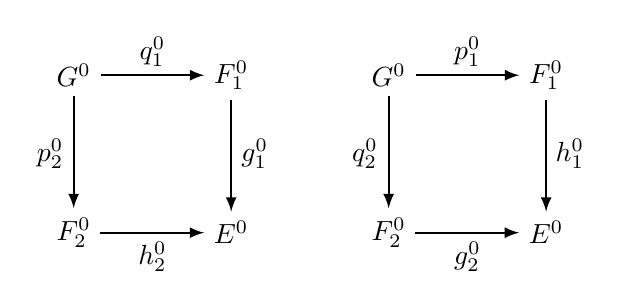
\begin{tikzpicture}[scale=1]
\node[] (A1) at (0,0) {$G^0$};
\node[] (A2) at (2,0) {$F_1^0$};
\node[] (A3) at (4,0) {$G^0$};
\node[] (A4) at (6,0) {$F_1^0$};

\node[] (B1) at (0,-2) {$F_2^0$};
\node[] (B2) at (2,-2) {$E^0$};
\node[] (B3) at (4,-2) {$F_2^0$};
\node[] (B4) at (6,-2) {$E^0$};


\path[->, >=latex,thick] (A1) edge [] node[]{} (A2);
\path[->, >=latex,thick] (B1) edge [] node[]{} (B2);
\path[->, >=latex,thick] (A3) edge [] node[]{} (A4);
\path[->, >=latex,thick] (B3) edge [] node[]{} (B4);

\path[->, >=latex,thick] (A1) edge [] node[]{} (B1);
\path[->, >=latex,thick] (A2) edge [] node[]{} (B2);
\path[->, >=latex,thick] (A3) edge [] node[]{} (B3);
\path[->, >=latex,thick] (A4) edge [] node[]{} (B4);

\node at (1,0.3) {$q_1^0$};
\node at (5,0.3) {$p_1^0$};
\node at (1,-2.3) {$h_2^0$};
\node at (5,-2.3) {$g_2^0$};

\node at (-0.3,-1) {$p_2^0$};
\node at (2.3,-1) {$g_1^0$};
\node at (3.7,-1) {$q_2^0$};
\node at (6.3,-1) {$h_1^0$};
\end{tikzpicture}
\]
are pullback squares;

$(iv)$ $q_1$ has $s$-path lifting. 

Then $q_1$ has unique $s$-path lifting and 

$(a)$ the diagrams 

\[
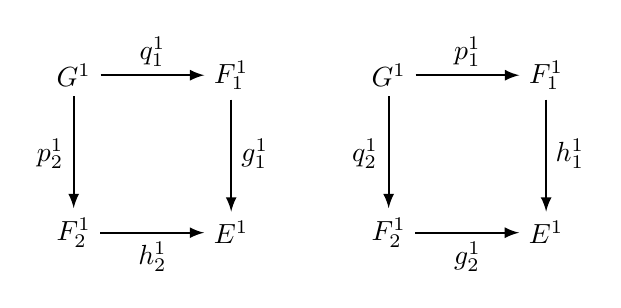
\begin{tikzpicture}[scale=1]
\node[] (A1) at (0,0) {$G^1$};
\node[] (A2) at (2,0) {$F_1^1$};
\node[] (A3) at (4,0) {$G^1$};
\node[] (A4) at (6,0) {$F_1^1$};

\node[] (B1) at (0,-2) {$F_2^1$};
\node[] (B2) at (2,-2) {$E^1$};
\node[] (B3) at (4,-2) {$F_2^1$};
\node[] (B4) at (6,-2) {$E^1$};


\path[->, >=latex,thick] (A1) edge [] node[]{} (A2);
\path[->, >=latex,thick] (B1) edge [] node[]{} (B2);
\path[->, >=latex,thick] (A3) edge [] node[]{} (A4);
\path[->, >=latex,thick] (B3) edge [] node[]{} (B4);

\path[->, >=latex,thick] (A1) edge [] node[]{} (B1);
\path[->, >=latex,thick] (A2) edge [] node[]{} (B2);
\path[->, >=latex,thick] (A3) edge [] node[]{} (B3);
\path[->, >=latex,thick] (A4) edge [] node[]{} (B4);

\node at (1,0.3) {$q_1^1$};
\node at (5,0.3) {$p_1^1$};
\node at (1,-2.3) {$h_2^1$};
\node at (5,-2.3) {$g_2^1$};

\node at (-0.3,-1) {$p_2^1$};
\node at (2.3,-1) {$g_1^1$};
\node at (3.7,-1) {$q_2^1$};
\node at (6.3,-1) {$h_1^1$};
\end{tikzpicture}
\]
are pullback squares;

$(b)$ $q_2$ has unique $s$-path lifting;

$(c)$ $p_1,p_2$ have unique $r$-path lifting.
\end{lem}

\begin{proof}
To show that the $s$-path lifting of $q_1$ is unique, consider $x,y\in G^1$ such that $s_G(x)=s_G(y)$ and $q_1^1(x)=q_1^1(y)$. Then \[s_{F_2}(p_2^1(x))=p_2^0(s_G(x))=p_2^0(s_G(y))=s_{F_2}(p_2^1(y)),\] and \[h_2^1(p_2^1(x))=g_1^1(q_1^1(x))=g_1^1(q_1^1(y))=h_2^1(p_2^1(y)).\] This implies $p_2^1(x)=p_2^1(y)$ by unique $s$-path lifting of $h_2$. A similar argument yields $q_2^1(x)=q_2^1(y)$. Again, \[s_{F_1}(p_1^1(x))=p_1^0(s_G(x))=p_1^0(s_G(y))=s_{F_1}(p_1^1(y)),\] and \[h_1^1(p_1^1(x))=g_2^1(q_2^1(x))=g_2^1(q_2^1(y))=h_1^1(p_1^1(y)),\] which gives $p_1^1(x)=p_1^1(y)$ by unique $s$-path lifting property of $h_1$. Similarly, using the first pullback square of $(iii)$, it can be shown that $r_G(x)=r_G(y)$. Since $s_G\times r_G\times p_1^1\times q_1^1\times p_2^1\times q_2^1$ is injective, we have $x=y$ and thus $q_1$ has unique $s$-path lifting. We now show that the first square in $(a)$ is a pullback square. For this, consider the following diagram:

\[
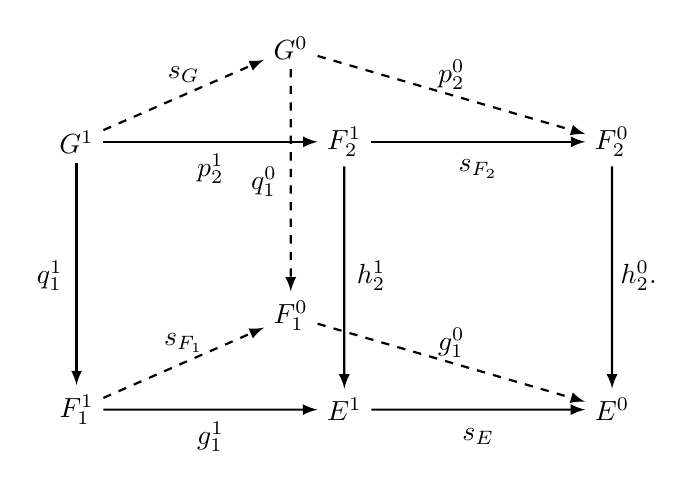
\begin{tikzpicture}[scale=1.7]
\node[] (A1) at (0,0) {$G^1$};
\node[] (A2) at (2,0) {$F_2^1$};
\node[] (A3) at (0,-2) {$F_1^1$};
\node[] (A4) at (2,-2) {$E^1$};

\node[] (B1) at (1.6,0.7) {$G^0$};
\node[] (B2) at (4,0) {$F_2^0$};
\node[] (B3) at (1.6,-1.3) {$F_1^0$};
\node[] (B4) at (4,-2) {$E^0$};

\path[->, black, >=latex,thick] (A1) edge [] node[]{} (A2);
\path[->, black, >=latex,thick] (A3) edge [] node[]{} (A4);
\path[->, black, >=latex,thick] (A1) edge [] node[]{} (A3);
\path[->, black, >=latex,thick] (A2) edge [] node[]{} (A4);

\path[->,black, dashed, >=latex,thick] (B1) edge [] node[]{} (B3);
\path[->,black, >=latex,thick] (A4) edge [] node[]{} (B4);
\path[->,black, >=latex,thick] (A2) edge [] node[]{} (B2);
\path[->,black, >=latex,thick] (B2) edge [] node[]{} (B4);

\path[->,black, dashed, >=latex,thick] (A1) edge [] node {} (B1);
\path[->,black, dashed, >=latex,thick] (A3) edge [] node {} (B3);
\path[->,black, dashed, >=latex,thick] (B1) edge [] node {} (B2);
\path[->,black, dashed, >=latex,thick] (B3) edge [] node {} (B4);

\node at (1,-0.2) {$p_2^1$};
\node at (1,-2.2) {$g_1^1$};
\node at (-0.2,-1) {$q_1^1$};
\node at (2.2,-1) {$h_2^1$};

\node at (3,-0.2) {$s_{F_2}$};
\node at (3,-2.2) {$s_E$};
\node at (4.2,-1) {$h_2^0$.};

\node at (0.8,0.5) {$s_G$};
\node at (0.8,-1.5) {$s_{F_1}$};
\node at (2.8,0.5) {$p_2^0$};
\node at (2.8,-1.5) {$g_1^0$};

\node at (1.4,-0.3) {$q_1^0$};

\end{tikzpicture}
\]
We observe that the two squares in the back are pullback squares. The right one is essentially the first square in $(iii)$, whereas the left one is a pullback square, since $q_1$ has unique $s$-path lifting. By pasting law for pullbacks, the rectangle in the back (formed by pasting the left and right squares, side by side) is a pullback rectangle. Now, $p_2$ and $g_1$ are graph morphisms, which implies $s_{F_2}\circ p_2^1=p_2^0\circ s_G$ and $s_E\circ g_1^1=g_1^0\circ s_{F_1}$. It follows that the rectangle in the front side, obtained by attaching the left and right squares along the side $h_2^1$ and then ignoring this side, is a pullback rectangle. Again, the right-hand square is a pullback due to the unique $s$-path lifting of $h_2$. Applying the pasting law again, we can conclude that the left-hand square is a pullback and we are done. 

Before tackling the second square in $(a)$, we prove $(b)$. Consider the diagram:

\[
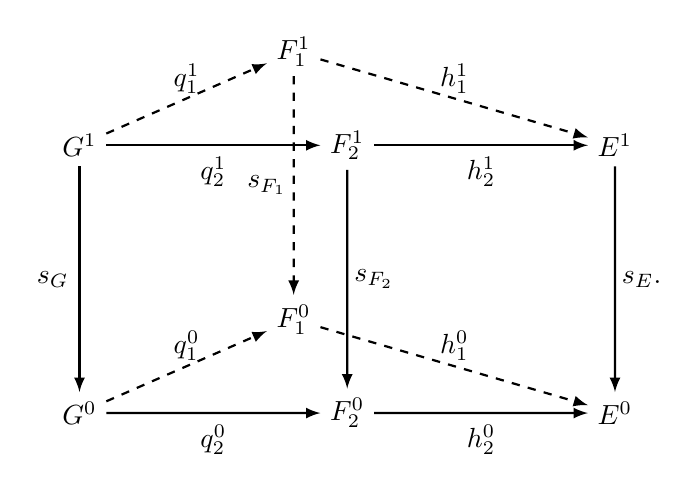
\begin{tikzpicture}[scale=1.7]
\node[] (A1) at (0,0) {$G^1$};
\node[] (A2) at (2,0) {$F_2^1$};
\node[] (A3) at (0,-2) {$G^0$};
\node[] (A4) at (2,-2) {$F_2^0$};

\node[] (B1) at (1.6,0.7) {$F_1^1$};
\node[] (B2) at (4,0) {$E^1$};
\node[] (B3) at (1.6,-1.3) {$F_1^0$};
\node[] (B4) at (4,-2) {$E^0$};

\path[->, black, >=latex,thick] (A1) edge [] node[]{} (A2);
\path[->, black, >=latex,thick] (A3) edge [] node[]{} (A4);
\path[->, black, >=latex,thick] (A1) edge [] node[]{} (A3);
\path[->, black, >=latex,thick] (A2) edge [] node[]{} (A4);

\path[->,black, dashed, >=latex,thick] (B1) edge [] node[]{} (B3);
\path[->,black, >=latex,thick] (A4) edge [] node[]{} (B4);
\path[->,black, >=latex,thick] (A2) edge [] node[]{} (B2);
\path[->,black, >=latex,thick] (B2) edge [] node[]{} (B4);

\path[->,black, dashed, >=latex,thick] (A1) edge [] node {} (B1);
\path[->,black, dashed, >=latex,thick] (A3) edge [] node {} (B3);
\path[->,black, dashed, >=latex,thick] (B1) edge [] node {} (B2);
\path[->,black, dashed, >=latex,thick] (B3) edge [] node {} (B4);

\node at (1,-0.2) {$q_2^1$};
\node at (1,-2.2) {$q_2^0$};
\node at (-0.2,-1) {$s_G$};
\node at (2.2,-1) {$s_{F_2}$};

\node at (3,-0.2) {$h_2^1$};
\node at (3,-2.2) {$h_2^0$};
\node at (4.2,-1) {$s_E$.};

\node at (0.8,0.5) {$q_1^1$};
\node at (0.8,-1.5) {$q_1^0$};
\node at (2.8,0.5) {$h_1^1$};
\node at (2.8,-1.5) {$h_1^0$};

\node at (1.4,-0.3) {$s_{F_1}$};

\end{tikzpicture}
\] Since $q_1,h_1$ have unique $s$-path lifting, the two squares in the back are pullback squares. Pasting these two along the side $s_{F_1}$, we have a pullback rectangle in the back. Note that, $h_1^1\circ q_1^1=h_2^1\circ q_2^1$ and $h_1^0\circ q_1^0=h_2^0\circ q_2^0$ by the inner-commutativity. Hence, the rectangle in the front (made with solid edges) is a pullback rectangle. Finally, since the right-hand square in the front is a pullback by the unique $s$-path lifting of $h_2$, it follows that the left-hand square is also a pullback whence, $q_2$ has unique $s$-path lifting. Now, with the unique $s$-path lifting of $q_2$ in hand, a similar line of argument, applied on the diagram:
\[
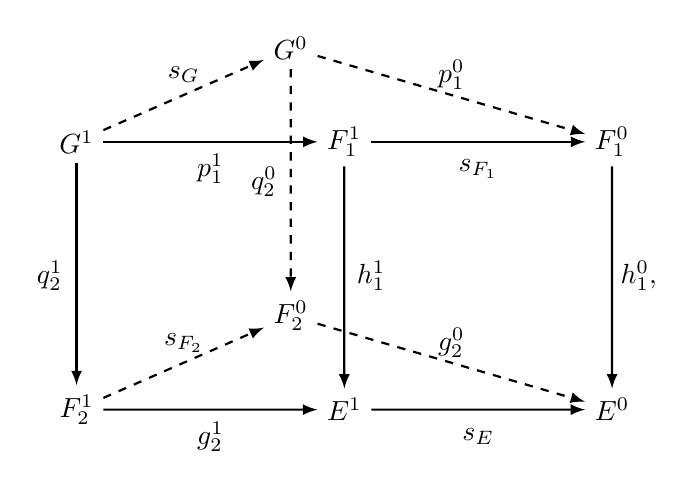
\begin{tikzpicture}[scale=1.7]
\node[] (A1) at (0,0) {$G^1$};
\node[] (A2) at (2,0) {$F_1^1$};
\node[] (A3) at (0,-2) {$F_2^1$};
\node[] (A4) at (2,-2) {$E^1$};

\node[] (B1) at (1.6,0.7) {$G^0$};
\node[] (B2) at (4,0) {$F_1^0$};
\node[] (B3) at (1.6,-1.3) {$F_2^0$};
\node[] (B4) at (4,-2) {$E^0$};

\path[->, black, >=latex,thick] (A1) edge [] node[]{} (A2);
\path[->, black, >=latex,thick] (A3) edge [] node[]{} (A4);
\path[->, black, >=latex,thick] (A1) edge [] node[]{} (A3);
\path[->, black, >=latex,thick] (A2) edge [] node[]{} (A4);

\path[->,black, dashed, >=latex,thick] (B1) edge [] node[]{} (B3);
\path[->,black, >=latex,thick] (A4) edge [] node[]{} (B4);
\path[->,black, >=latex,thick] (A2) edge [] node[]{} (B2);
\path[->,black, >=latex,thick] (B2) edge [] node[]{} (B4);

\path[->,black, dashed, >=latex,thick] (A1) edge [] node {} (B1);
\path[->,black, dashed, >=latex,thick] (A3) edge [] node {} (B3);
\path[->,black, dashed, >=latex,thick] (B1) edge [] node {} (B2);
\path[->,black, dashed, >=latex,thick] (B3) edge [] node {} (B4);

\node at (1,-0.2) {$p_1^1$};
\node at (1,-2.2) {$g_2^1$};
\node at (-0.2,-1) {$q_2^1$};
\node at (2.2,-1) {$h_1^1$};

\node at (3,-0.2) {$s_{F_1}$};
\node at (3,-2.2) {$s_E$};
\node at (4.2,-1) {$h_1^0$,};

\node at (0.8,0.5) {$s_G$};
\node at (0.8,-1.5) {$s_{F_2}$};
\node at (2.8,0.5) {$p_1^0$};
\node at (2.8,-1.5) {$g_2^0$};

\node at (1.4,-0.3) {$q_2^0$};

\end{tikzpicture}
\] shows that the second square in $(a)$ is a pullback. Again, using this pullback square, it can be shown that $p_1$ has unique $r$-path lifting, for which one needs to apply similar order of reasoning on the diagram:

\[
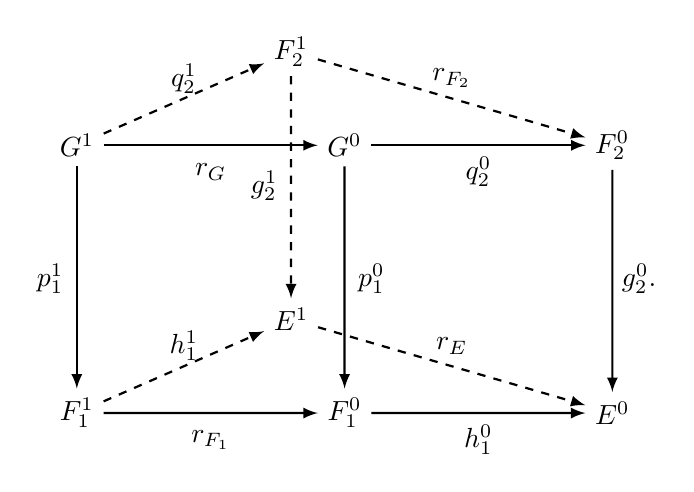
\begin{tikzpicture}[scale=1.7]
\node[] (A1) at (0,0) {$G^1$};
\node[] (A2) at (2,0) {$G^0$};
\node[] (A3) at (0,-2) {$F_1^1$};
\node[] (A4) at (2,-2) {$F_1^0$};

\node[] (B1) at (1.6,0.7) {$F_2^1$};
\node[] (B2) at (4,0) {$F_2^0$};
\node[] (B3) at (1.6,-1.3) {$E^1$};
\node[] (B4) at (4,-2) {$E^0$};

\path[->, black, >=latex,thick] (A1) edge [] node[]{} (A2);
\path[->, black, >=latex,thick] (A3) edge [] node[]{} (A4);
\path[->, black, >=latex,thick] (A1) edge [] node[]{} (A3);
\path[->, black, >=latex,thick] (A2) edge [] node[]{} (A4);

\path[->,black, dashed, >=latex,thick] (B1) edge [] node[]{} (B3);
\path[->,black, >=latex,thick] (A4) edge [] node[]{} (B4);
\path[->,black, >=latex,thick] (A2) edge [] node[]{} (B2);
\path[->,black, >=latex,thick] (B2) edge [] node[]{} (B4);

\path[->,black, dashed, >=latex,thick] (A1) edge [] node {} (B1);
\path[->,black, dashed, >=latex,thick] (A3) edge [] node {} (B3);
\path[->,black, dashed, >=latex,thick] (B1) edge [] node {} (B2);
\path[->,black, dashed, >=latex,thick] (B3) edge [] node {} (B4);

\node at (1,-0.2) {$r_G$};
\node at (1,-2.2) {$r_{F_1}$};
\node at (-0.2,-1) {$p_1^1$};
\node at (2.2,-1) {$p_1^0$};

\node at (3,-0.2) {$q_2^0$};
\node at (3,-2.2) {$h_1^0$};
\node at (4.2,-1) {$g_2^0$.};

\node at (0.8,0.5) {$q_2^1$};
\node at (0.8,-1.5) {$h_1^1$};
\node at (2.8,0.5) {$r_{F_2}$};
\node at (2.8,-1.5) {$r_E$};

\node at (1.4,-0.3) {$g_2^1$};

\end{tikzpicture}
\] Finally, interchanging the subscripts $1$ and $2$ at relevant nodes and arrows in the above diagram, and using necessary pullbacks in the resulting diagram, we can show that $p_2$ has unique $r$-path lifting. 
\end{proof}

\end{document}
